% =====================================================================
% Artigo do projeto final: detecção de voz deepfake em PT-BR com CNN
% Template JBCS/SBC (sbc2023).
%
% COMO USAR NO OVERLEAF
%  1. Crie o projeto a partir do template JBCS (ele traz sbc2023.cls e
%     apalike-sol.bst).
%  2. Substitua todo o conteúdo do .tex principal por este arquivo.
%  3. Crie a pasta "figuras" no projeto (ícone de nova pasta) e envie para
%     ela as 8 imagens de documentacao/figuras/ (gráficos do Colab).
%  4. Menu -> Compiler -> XeLaTeX (o template usa fontspec; pdfLaTeX falha).
%
% As referências estão no bloco filecontents* abaixo: o próprio arquivo
% grava o refs.bib. Se o seu LaTeX reclamar do [overwrite], copie o
% conteúdo do bloco para um arquivo refs.bib e apague o bloco.
% =====================================================================
\begin{filecontents*}[overwrite]{refs.bib}
@inproceedings{todisco2019asvspoof,
  author    = {Todisco, Massimiliano and Wang, Xin and Vestman, Ville and Sahidullah, Md and Delgado, H{\'e}ctor and Nautsch, Andreas and Yamagishi, Junichi and Evans, Nicholas and Kinnunen, Tomi and Lee, Kong Aik},
  title     = {{ASVspoof} 2019: Future Horizons in Spoofed and Fake Audio Detection},
  booktitle = {Proc. Interspeech},
  pages     = {1008--1012},
  year      = {2019}
}
@article{liu2023asvspoof2021,
  author  = {Liu, Xuechen and Wang, Xin and Sahidullah, Md and Patino, Jose and Delgado, H{\'e}ctor and Kinnunen, Tomi and Todisco, Massimiliano and Yamagishi, Junichi and Evans, Nicholas and Nautsch, Andreas and Lee, Kong Aik},
  title   = {{ASVspoof} 2021: Towards Spoofed and Deepfake Speech Detection in the Wild},
  journal = {IEEE/ACM Transactions on Audio, Speech, and Language Processing},
  volume  = {31},
  pages   = {2507--2522},
  year    = {2023}
}
@inproceedings{muller2022itw,
  author    = {M{\"u}ller, Nicolas M. and Czempin, Pavel and Dieckmann, Franziska and Froghyar, Adam and B{\"o}ttinger, Konstantin},
  title     = {Does Audio Deepfake Detection Generalize?},
  booktitle = {Proc. Interspeech},
  pages     = {2783--2787},
  year      = {2022}
}
@inproceedings{muller2024mlaad,
  author    = {M{\"u}ller, Nicolas M. and Kawa, Piotr and Choong, Wei Herng and Casanova, Edresson and G{\"o}lge, Eren and M{\"u}ller, Thorsten and Syga, Piotr and Sperl, Philip and B{\"o}ttinger, Konstantin},
  title     = {{MLAAD}: The Multi-Language Audio Anti-Spoofing Dataset},
  booktitle = {International Joint Conference on Neural Networks (IJCNN)},
  year      = {2024}
}
@inproceedings{sahidullah2015features,
  author    = {Sahidullah, Md and Kinnunen, Tomi and Hanil{\c{c}}i, Cemal},
  title     = {A Comparison of Features for Synthetic Speech Detection},
  booktitle = {Proc. Interspeech},
  pages     = {2087--2091},
  year      = {2015}
}
@inproceedings{lavrentyev2019stc,
  author    = {Lavrentyeva, Galina and Novoselov, Sergey and Tseren, Andzhukaev and Volkova, Marina and Gorlanov, Artem and Kozlov, Alexandr},
  title     = {{STC} Antispoofing Systems for the {ASVspoof2019} Challenge},
  booktitle = {Proc. Interspeech},
  pages     = {1033--1037},
  year      = {2019}
}
@article{kong2020panns,
  author  = {Kong, Qiuqiang and Cao, Yin and Iqbal, Turab and Wang, Yuxuan and Wang, Wenwu and Plumbley, Mark D.},
  title   = {{PANNs}: Large-Scale Pretrained Audio Neural Networks for Audio Pattern Recognition},
  journal = {IEEE/ACM Transactions on Audio, Speech, and Language Processing},
  volume  = {28},
  pages   = {2880--2894},
  year    = {2020}
}
@inproceedings{he2016resnet,
  author    = {He, Kaiming and Zhang, Xiangyu and Ren, Shaoqing and Sun, Jian},
  title     = {Deep Residual Learning for Image Recognition},
  booktitle = {IEEE Conference on Computer Vision and Pattern Recognition (CVPR)},
  pages     = {770--778},
  year      = {2016}
}
@inproceedings{park2019specaugment,
  author    = {Park, Daniel S. and Chan, William and Zhang, Yu and Chiu, Chung-Cheng and Zoph, Barret and Cubuk, Ekin D. and Le, Quoc V.},
  title     = {{SpecAugment}: A Simple Data Augmentation Method for Automatic Speech Recognition},
  booktitle = {Proc. Interspeech},
  pages     = {2613--2617},
  year      = {2019}
}
@inproceedings{ardila2020commonvoice,
  author    = {Ardila, Rosana and Branson, Megan and Davis, Kelly and Kohler, Michael and Meyer, Josh and Henretty, Michael and Morais, Reuben and Saunders, Lindsay and Tyers, Francis and Weber, Gregor},
  title     = {Common Voice: A Massively-Multilingual Speech Corpus},
  booktitle = {Proc. Language Resources and Evaluation Conference (LREC)},
  pages     = {4218--4222},
  year      = {2020}
}
@inproceedings{ioffe2015batchnorm,
  author    = {Ioffe, Sergey and Szegedy, Christian},
  title     = {Batch Normalization: Accelerating Deep Network Training by Reducing Internal Covariate Shift},
  booktitle = {International Conference on Machine Learning (ICML)},
  pages     = {448--456},
  year      = {2015}
}
@article{srivastava2014dropout,
  author  = {Srivastava, Nitish and Hinton, Geoffrey and Krizhevsky, Alex and Sutskever, Ilya and Salakhutdinov, Ruslan},
  title   = {Dropout: A Simple Way to Prevent Neural Networks from Overfitting},
  journal = {Journal of Machine Learning Research},
  volume  = {15},
  pages   = {1929--1958},
  year    = {2014}
}
@inproceedings{kingma2015adam,
  author    = {Kingma, Diederik P. and Ba, Jimmy},
  title     = {Adam: A Method for Stochastic Optimization},
  booktitle = {International Conference on Learning Representations (ICLR)},
  year      = {2015}
}
@inproceedings{loshchilov2019adamw,
  author    = {Loshchilov, Ilya and Hutter, Frank},
  title     = {Decoupled Weight Decay Regularization},
  booktitle = {International Conference on Learning Representations (ICLR)},
  year      = {2019}
}
@inproceedings{loshchilov2017sgdr,
  author    = {Loshchilov, Ilya and Hutter, Frank},
  title     = {{SGDR}: Stochastic Gradient Descent with Warm Restarts},
  booktitle = {International Conference on Learning Representations (ICLR)},
  year      = {2017}
}
@inproceedings{szegedy2016inception,
  author    = {Szegedy, Christian and Vanhoucke, Vincent and Ioffe, Sergey and Shlens, Jon and Wojna, Zbigniew},
  title     = {Rethinking the Inception Architecture for Computer Vision},
  booktitle = {IEEE Conference on Computer Vision and Pattern Recognition (CVPR)},
  pages     = {2818--2826},
  year      = {2016}
}
@inproceedings{mcfee2015librosa,
  author    = {McFee, Brian and Raffel, Colin and Liang, Dawen and Ellis, Daniel P. W. and McVicar, Matt and Battenberg, Eric and Nieto, Oriol},
  title     = {librosa: Audio and Music Signal Analysis in Python},
  booktitle = {Proc. 14th Python in Science Conference (SciPy)},
  pages     = {18--25},
  year      = {2015}
}
@misc{abadi2016tensorflow,
  author = {Abadi, Mart{\'\i}n and others},
  title  = {{TensorFlow}: Large-Scale Machine Learning on Heterogeneous Systems},
  year   = {2015},
  note   = {Software dispon{\'\i}vel em \url{https://www.tensorflow.org}}
}
@article{pedregosa2011sklearn,
  author  = {Pedregosa, Fabian and others},
  title   = {Scikit-learn: Machine Learning in {P}ython},
  journal = {Journal of Machine Learning Research},
  volume  = {12},
  pages   = {2825--2830},
  year    = {2011}
}
@misc{coraamupe,
  author       = {{NILC-NLP}},
  title        = {{CORAA-MUPE-ASR}: corpus de entrevistas em portugu{\^e}s brasileiro},
  howpublished = {\url{https://huggingface.co/datasets/nilc-nlp/CORAA-MUPE-ASR}},
  note         = {Acesso em: out. 2026},
  year         = {2026}
}
@misc{commonvoice17hf,
  author       = {{Fixie AI}},
  title        = {Common Voice 17.0 (espelho no Hugging Face)},
  howpublished = {\url{https://huggingface.co/datasets/fixie-ai/common_voice_17_0}},
  note         = {Acesso em: out. 2026},
  year         = {2026}
}
@misc{stafford2024deepfake,
  author       = {Stafford, Gary A.},
  title        = {Deepfake Audio Detection Dataset},
  howpublished = {\url{https://huggingface.co/datasets/garystafford/deepfake-audio-detection}},
  note         = {Acesso em: out. 2026},
  year         = {2026}
}
@misc{brspeechdf,
  author       = {{AKCIT}},
  title        = {{BRSpeech-DF}: Brazilian Portuguese Speech Deepfake Dataset},
  howpublished = {\url{https://huggingface.co/datasets/AKCIT-Deepfake/BRSpeech-DF}},
  note         = {Acesso em: out. 2026},
  year         = {2026}
}
@misc{edgetts,
  author       = {{rany2}},
  title        = {edge-tts: use o servi{\c{c}}o de TTS do Microsoft Edge a partir do Python},
  howpublished = {\url{https://github.com/rany2/edge-tts}},
  note         = {Acesso em: out. 2026},
  year         = {2026}
}
@misc{gtts,
  author       = {Durette, Pierre Nicolas},
  title        = {{gTTS}: Google Text-to-Speech},
  howpublished = {\url{https://github.com/pndurette/gTTS}},
  note         = {Acesso em: out. 2026},
  year         = {2026}
}
\end{filecontents*}
\documentclass{sbc2023}%

\usepackage{graphicx}
%\usepackage[utf8]{inputenc}
\usepackage[misc,geometry]{ifsym}
\usepackage{fontspec}
\usepackage[brazilian]{babel} % hifenização em português (não está no template)
\usepackage{fontawesome}
\usepackage{academicons}
\usepackage{color}
\usepackage{hyperref}
\usepackage{aas_macros}
\usepackage[bottom]{footmisc}
\usepackage{supertabular}
\usepackage{afterpage}
\usepackage{url}
\usepackage{pifont}
\usepackage{multicol}
\usepackage{multirow}

\setcitestyle{square}

% Rótulos em português (a classe usa os nomes em inglês)
\AtBeginDocument{%
  \renewcommand{\tablename}{Tabela}%
  \renewcommand{\figurename}{Figura}%
  \renewcommand{\refname}{Referências}}

\definecolor{orcidlogo}{rgb}{0.37,0.48,0.13}
\definecolor{unilogo}{rgb}{0.16, 0.26, 0.58}
\definecolor{maillogo}{rgb}{0.58, 0.16, 0.26}
\definecolor{darkblue}{rgb}{0.0,0.0,0.0}
\hypersetup{colorlinks,breaklinks,
            linkcolor=darkblue,urlcolor=darkblue,
            anchorcolor=darkblue,citecolor=darkblue}
%\hypersetup{colorlinks,citecolor=blue,linkcolor=blue,urlcolor=blue}

%%%%%%% IMPORTANT: We disable hyperlinks by default with this line, to avoid the error "\pdfendlink ended up in different nesting level" while writing.
%\hypersetup{draft}

\jid{UTFPR}
\jtitle{Projeto Final da disciplina de Aprendizado Profundo, UTFPR, 2026, }
\doi{N/A}
\copyrightstatement{This work is licensed under a Creative Commons Attribution 4.0 International License}
\jyear{2026}


\title[Detecção de voz deepfake em PT-BR com CNN]{Detecção de voz deepfake em português brasileiro com redes neurais convolucionais robustas a canal e a vozes comerciais}

\author[Portella e Silva 2026]{
\affil{\textbf{Carlos Eduardo Rosa Portella}~~[~\textbf{Universidade Tecnológica Federal do Paraná, Campus Curitiba}~|\href{mailto:carlosportella@alunos.utfpr.edu.br}{~\textbf{\textit{carlosportella@alunos.utfpr.edu.br}}}~]}

\affil{\textbf{Felipe Pereira da Silva}~~[~\textbf{Universidade Tecnológica Federal do Paraná, Campus Curitiba}~|\href{mailto:fsilva.2026@alunos.utfpr.edu.br}{~\textbf{\textit{fsilva.2026@alunos.utfpr.edu.br}}}~]}

}

\begin{document}

\begin{frontmatter}
\maketitle

% Sem o ambiente mail: a classe põe um ícone de e-mail antes do endereço,
% e a instituição e o campus já aparecem na linha de cada autor.

\begin{dates}
\small{\textbf{Entregue em:} 18 de outubro de 2026~~~$\bullet$~~~\textbf{Disciplina:} Aprendizado Profundo (\textit{Deep Learning})~~~$\bullet$~~~\textbf{Professora:} Mariana Antonia Aguiar Furucho (\href{mailto:marianafurucho@utfpr.edu.br}{marianafurucho@utfpr.edu.br})}

\end{dates}


\begin{abstract}
\textbf{Resumo.~}
\noindent Ferramentas comerciais de clonagem de voz, como o ElevenLabs, produzem falas sintéticas difíceis de distinguir das reais, e detectores treinados só com bases acadêmicas costumam falhar diante delas. Este trabalho apresenta um detector de voz deepfake em português brasileiro baseado em uma rede neural convolucional (CNN) treinada do zero sobre espectrogramas log-mel. O treino combina falsos de 16 sintetizadores do MLAAD, falsos comerciais (ElevenLabs, Amazon Polly, Microsoft Edge TTS, Google TTS, entre outros) e falas reais do CORAA-MUPE e do Common Voice, com idiomas balanceados entre as classes. Para que o modelo funcione em áudios do dia a dia, cada exemplo recebe codecs com perdas, uma cadeia que imita o reenvio pelo WhatsApp e degradações de canal, aplicados igualmente a reais e falsos. O modelo final, um ensemble de duas CNNs residuais com 501.953 parâmetros cada, treinado no Google Colab, obteve EER de 1,75\% no teste limpo, 6,5\% no teste degradado e 1,25\% em sintetizadores nunca vistos no treino. Em um teste cego com áudios gravados e gerados pelo próprio grupo, detectou 13 de 16 falsos e acertou os 9 reais. Os resultados foram reproduzidos em um Mac mini M4, com diferenças de até 1,8 ponto de EER. O desempenho em áudios coletados da internet (In-the-Wild, EER de 30,6\%) mostra o limite atual da abordagem.

\medskip
\textbf{Abstract.~}
\noindent Commercial voice-cloning tools such as ElevenLabs produce synthetic speech that is hard to tell apart from real speech, and detectors trained only on academic corpora often fail on it. This work presents a Brazilian Portuguese voice deepfake detector based on a convolutional neural network (CNN) trained from scratch on log-mel spectrograms. Training combines fakes from 16 MLAAD synthesizers, commercial fakes (ElevenLabs, Amazon Polly, Microsoft Edge TTS, Google TTS, among others) and real speech from CORAA-MUPE and Common Voice, with languages balanced across classes. To make the model work on everyday recordings, every example goes through lossy codecs, a chain that mimics WhatsApp forwarding, and channel degradations, applied equally to both classes. The final model, an ensemble of two residual CNNs with 501,953 parameters each, trained on Google Colab, reached an EER of 1.75\% on the clean test set, 6.5\% on the degraded test set and 1.25\% on synthesizers never seen in training. On a blind test with audio recorded and generated by the authors, it detected 13 of 16 fakes and classified all 9 real recordings correctly. The results were reproduced on a Mac mini M4, with EER differences of up to 1.8 points. Performance on audio collected from the internet (In-the-Wild, 30.6\% EER) shows the current limit of the approach.
\end{abstract}

\begin{keywords}
Deepfake de voz, Detecção de falsificação, Redes neurais convolucionais, Espectrograma log-mel, Português brasileiro
\end{keywords}

\end{frontmatter}


\section{Introdução}
\label{sec:intro}

A síntese de voz por redes neurais tornou-se acessível a qualquer pessoa. Serviços comerciais clonam uma voz a partir de poucos segundos de áudio e produzem falas naturais em português, o que abre espaço para golpes por telefone, mensagens de áudio falsas e desinformação. Detectar automaticamente se uma fala é real ou sintética é, portanto, um problema prático, e não apenas acadêmico.

A área de detecção de falsificação de voz (\textit{anti-spoofing}) evoluiu com as competições ASVspoof~\citep{todisco2019asvspoof,liu2023asvspoof2021}, que fornecem bases padronizadas e métricas como a taxa de erro igual (EER). Entretanto, modelos com ótimo desempenho nessas bases perdem muito quando avaliados em áudios reais da internet~\citep{muller2022itw}, e as bases disponíveis são majoritariamente em inglês.

Este trabalho partiu de uma versão inicial do projeto em que o detector não reconhecia vozes geradas por serviços comerciais como o ElevenLabs. O objetivo foi construir um detector que: (i) classifique áudios em português brasileiro em qualquer formato comum (MP3, WAV, Ogg/Opus do WhatsApp, M4A etc.); (ii) reconheça vozes de serviços comerciais; (iii) seja robusto a compressão e a degradações de canal; e (iv) possa ser treinado em um computador pessoal (Mac mini M4) e reproduzido no Google Colab. Por exigência da disciplina, o modelo é uma CNN pura em Keras, treinada do zero.

As principais contribuições são:
\begin{itemize}
\item uma combinação de bases públicas com falsos comerciais e idiomas balanceados entre as classes, para que nem o idioma nem o gerador sejam atalhos para a resposta;
\item um esquema de aumento de dados que aplica os mesmos codecs e degradações às duas classes, incluindo uma cadeia que imita o reenvio pelo WhatsApp;
\item uma avaliação em cinco conjuntos (limpo, degradado, sintetizadores nunca vistos, generalização degradada e In-the-Wild), mais um teste cego com áudios do próprio grupo;
\item um registro das decisões tomadas, com os experimentos que não melhoraram o modelo.
\end{itemize}

O restante do texto está organizado assim: a Seção~\ref{sec:relacionados} resume os trabalhos relacionados; a Seção~\ref{sec:dados} descreve as bases; a Seção~\ref{sec:metodo}, o método; a Seção~\ref{sec:resultados}, os experimentos e resultados; a Seção~\ref{sec:discussao} discute as limitações; a Seção~\ref{sec:etica} trata das questões éticas; e a Seção~\ref{sec:conclusao} conclui.


\section{Trabalhos relacionados}
\label{sec:relacionados}

As competições ASVspoof 2019 e 2021~\citep{todisco2019asvspoof,liu2023asvspoof2021} consolidaram a detecção de fala sintética como tarefa de classificação binária avaliada por EER. Entre as características acústicas, os coeficientes cepstrais em escala linear (LFCC) mostraram bom desempenho em detecção de fala sintética~\citep{sahidullah2015features}, e as CNNs leves com ativação \textit{Max-Feature-Map} (LCNN) estiveram entre os melhores sistemas do ASVspoof 2019~\citep{lavrentyev2019stc}.

\citet{muller2022itw} mostraram que esses modelos generalizam mal: ao serem avaliados no conjunto In-the-Wild, composto por áudios de figuras públicas coletados da internet, o EER sobe drasticamente. Para ampliar a cobertura de idiomas e de sintetizadores, os mesmos autores publicaram o MLAAD~\citep{muller2024mlaad}, com falsos gerados por dezenas de modelos de síntese em vários idiomas, incluindo o português.

Redes pré-treinadas em grandes volumes de áudio, como as PANNs~\citep{kong2020panns}, são uma alternativa à rede treinada do zero, e foram testadas neste trabalho como comparação. A arquitetura escolhida usa conexões residuais~\citep{he2016resnet}, e o aumento de dados inclui o SpecAugment~\citep{park2019specaugment}.


\section{Bases de dados}
\label{sec:dados}

Todas as bases são públicas e baixadas automaticamente pelo código (Tabela~\ref{tab:bases}). Os falsos de três sintetizadores do MLAAD (OpenAI TTS-1 HD, Voxtral e Qwen3-TTS 1.7B) foram reservados exclusivamente para o teste de generalização. O In-the-Wild é usado apenas na avaliação e nunca entra no treino nem na escolha do limiar.

\begin{table*}[!ht]
\caption{Bases de dados utilizadas.}
\centering
\small
\begin{tabular}{@{}p{3.3cm}p{9.0cm}p{3.2cm}@{}}
\hline\hline
Base & Uso no projeto & Licença \\
\hline
MLAAD~\citep{muller2024mlaad} & Falsos de 16 sintetizadores em português (3 reservados à generalização) e, em 20\% dos falsos, geradores de outros idiomas (en, es, de, fr, it) como ElevenLabs v2/v3/Turbo, Cartesia, MiniMax e Bark & CC BY-NC 4.0 \\
Deepfake Audio Detection~\citep{stafford2024deepfake} & Falsos comerciais (ElevenLabs, Amazon Polly, Speechify, Hume AI, Luvvoice, Kokoro) e reais do YouTube, em inglês & CC BY 4.0 \\
Microsoft Edge TTS~\citep{edgetts} e gTTS~\citep{gtts} & Falsos comerciais gerados pelo código, com vozes neurais pt-BR e pt-PT & --- \\
CORAA-MUPE~\citep{coraamupe} & Reais: entrevistas em português brasileiro & ver página da base \\
Common Voice 17~\citep{ardila2020commonvoice,commonvoice17hf} & Reais gravados por voluntários (celular e notebook) em português e nos mesmos idiomas dos falsos estrangeiros; também fornece as frases lidas pelo Edge TTS e pelo gTTS & CC0 \\
In-the-Wild~\citep{muller2022itw} & Só avaliação: 400 falsos e 400 reais de figuras públicas, coletados da internet, em inglês & CC BY-SA 4.0 \\
BRSpeech-DF~\citep{brspeechdf} & Avaliada e descartada (Seção~\ref{sec:descartados}) & ver página da base \\
\hline\hline
\end{tabular}
\label{tab:bases}
\end{table*}

O treino usa 8.000 áudios (4.000 por classe). A validação e o teste têm 400 áudios por classe cada, e o teste de generalização tem 200 por classe. A divisão entre treino, validação e teste é fixa por arquivo, feita pelo \textit{hash} MD5 do nome, de modo que nenhum arquivo aparece em mais de um conjunto.

Para que o idioma não denuncie a classe, os falsos em inglês e em outros idiomas entram acompanhados de reais dos mesmos idiomas, na mesma proporção. Uma verificação automática interrompe a execução se a diferença de proporção de qualquer idioma entre reais e falsos passar de 5 pontos percentuais em algum conjunto. As cotas de cada gerador são distribuídas pelo método do maior resto, e a cota que um gerador pequeno não consegue preencher é repassada aos demais. O Bark, o gerador menos detectado nos primeiros experimentos, recebe cota dobrada.

\paragraph{Áudios do grupo.} O grupo reuniu 16 áudios falsos, gerados majoritariamente no ElevenLabs, e 9 gravações reais enviadas pelo WhatsApp. Esses 25 arquivos nunca são usados no treino nem na escolha do limiar e formam o teste cego, tratado como a métrica final do projeto.


\section{Metodologia}
\label{sec:metodo}

\subsection{Pré-processamento}

Todo áudio é decodificado com o \texttt{ffmpeg}, o que permite aceitar MP3, WAV, Ogg/Opus, M4A, AAC, FLAC, WebM e MP4, e convertido para mono, 16~kHz. A taxa de 16~kHz foi escolhida porque, acima de 8~kHz de frequência, os codecs cortam o espectro de formas diferentes (o Opus em torno de 12~kHz, o ElevenLabs em torno de 15~kHz), e essa faixa daria ao modelo um atalho pela largura de banda. Em seguida, os silêncios das pontas são removidos (limiar de 35~dB abaixo do pico) e o pico é normalizado em 0,95. Áudios com menos de 1~s de fala são rejeitados.

O áudio é dividido em janelas de 3~s com passo de 1,5~s, cobrindo o arquivo inteiro. Áudios curtos são repetidos até 3~s, em vez de preenchidos com silêncio. Cada janela é convertida em um espectrograma log-mel: STFT com janela de Hann de 1.024 pontos e passo de 160 amostras (10~ms), 128 filtros mel entre 20~Hz e 8~kHz, potência em dB com faixa de 80~dB e escala final em $[0,1]$. A entrada da rede tem, portanto, dimensão $128 \times 301 \times 1$.

\subsection{Aumento de dados e proteções contra atalhos}

Um detector pode aprender pistas que não têm relação com a síntese da voz, como o formato do arquivo, o nível de ruído de fundo ou o idioma. Para evitar isso, todas as transformações abaixo são sorteadas sem olhar o rótulo, com a mesma probabilidade para reais e falsos:
\begin{itemize}
\item \textbf{Três versões por áudio:} cada áudio de treino tem três versões independentes, cada uma com recorte, codec e degradação próprios, e uma delas é sorteada a cada época.
\item \textbf{Codec com perdas} ($p=0{,}7$): ida e volta por MP3 (24--128~kbps), Opus (12--32~kbps) ou AAC (32--128~kbps).
\item \textbf{Reenvio pelo WhatsApp} (25\% dos codecs): Opus a 16--32~kbps, seguido de MP3 ou AAC a 24~kHz e 32--64~kbps.
\item \textbf{Degradações de canal} ($p=0{,}5$; uma ou duas por trecho): banda telefônica (300--3.400~Hz), ruído branco com SNR de 10--35~dB, reverberação sintética (RT60 de 0,15--0,6~s), filtro passa-baixa (corte de 3,5--7,5~kHz) e equalização aleatória ($\pm$6~dB).
\item \textbf{Ruído de fundo emprestado} ($p=0{,}7$): o piso de ruído de um áudio real sorteado é aplicado aos falsos, para que ``silêncio limpo'' não vire pista de voz sintética.
\item \textbf{SpecAugment}~\citep{park2019specaugment}: durante o treino, uma faixa de até 12 bandas de frequência e outra de até 30 quadros (0,3~s) são zeradas em cada amostra.
\end{itemize}

A Figura~\ref{fig:espectrogramas} mostra a entrada da rede para um áudio real e um falso, antes e depois da degradação. No exemplo, a degradação do falso corta as bandas mais altas e adiciona ruído de fundo. Como o mesmo tipo de transformação é aplicado aos reais, a rede não pode usar a ausência de ruído ou a largura de banda como pista.

\begin{figure*}[!ht]
\begin{center}
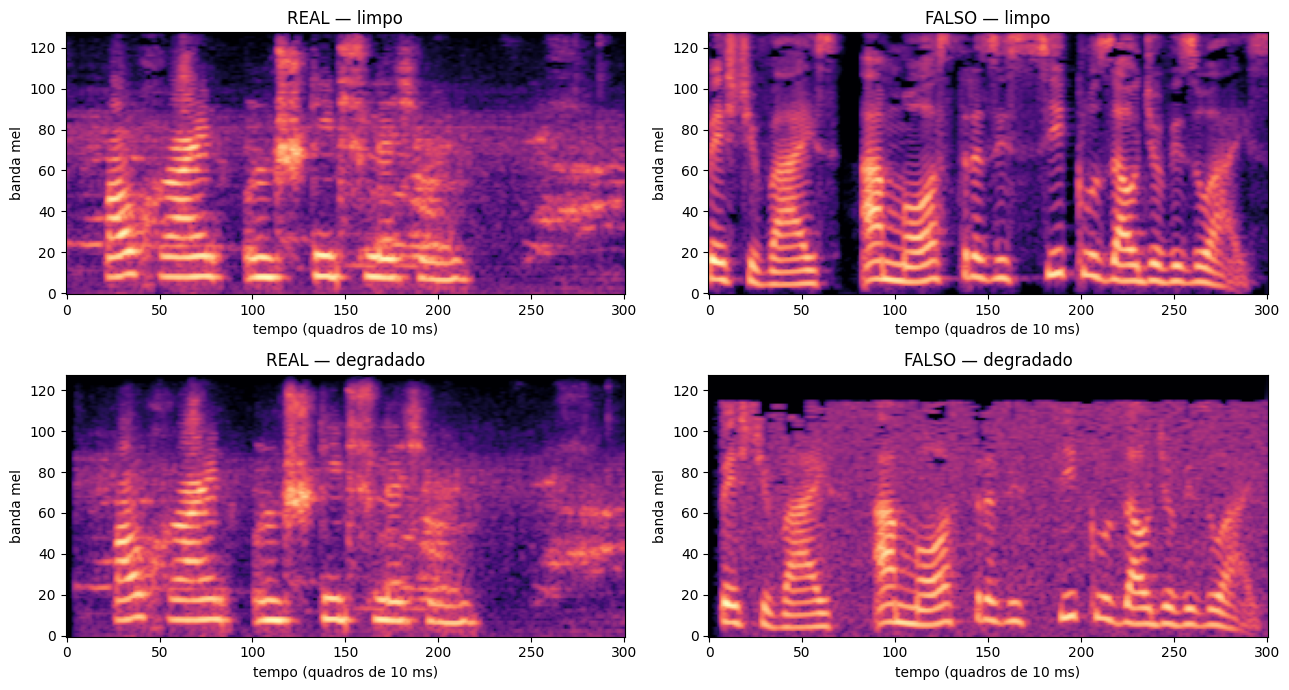
\includegraphics[width=0.85\textwidth]{figuras/espectrogramas.png}
\caption{Espectrogramas log-mel ($128 \times 301$) de um trecho real e de um falso, limpos e degradados, como gerados no Colab.}
\label{fig:espectrogramas}
\end{center}
\end{figure*}

\subsection{Arquitetura}

A CNN tem quatro blocos residuais~\citep{he2016resnet} com 32, 64, 96 e 128 filtros (Tabela~\ref{tab:arquitetura}). Cada bloco aplica duas convoluções $3 \times 3$ com normalização em lote~\citep{ioffe2015batchnorm} e soma o resultado a um atalho (convolução $1 \times 1$ quando o número de canais muda). Após cada bloco vêm um \textit{max pooling} $2 \times 2$ e um \textit{dropout} espacial de 10\%. No fim, a média global e o máximo global de cada mapa são concatenados. O máximo captura artefatos de síntese localizados, que a média diluiria. Uma camada densa com regularização L2 e \textit{dropout} de 40\%~\citep{srivastava2014dropout} precede a saída sigmoide, que fornece a probabilidade de o trecho ser falso, $P(\text{fake})$.

\begin{table*}[!ht]
\caption{Arquitetura de cada CNN residual do ensemble (501.953 parâmetros).}
\centering
\small
\begin{tabular}{@{}p{3.2cm}p{9.6cm}p{2.6cm}@{}}
\hline\hline
Camada & Configuração & Saída \\
\hline
Entrada & espectrograma log-mel & $128 \times 301 \times 1$ \\
Bloco residual 1 & Conv $3 \times 3$ (32) $\rightarrow$ BN $\rightarrow$ ReLU $\rightarrow$ Conv $3 \times 3$ $\rightarrow$ BN, somado ao atalho (Conv $1 \times 1$ + BN) $\rightarrow$ ReLU $\rightarrow$ MaxPool $2 \times 2$ $\rightarrow$ SpatialDropout 10\% & $64 \times 150 \times 32$ \\
Bloco residual 2 & idem, 64 filtros & $32 \times 75 \times 64$ \\
Bloco residual 3 & idem, 96 filtros & $16 \times 37 \times 96$ \\
Bloco residual 4 & idem, 128 filtros & $8 \times 18 \times 128$ \\
Pooling global & GlobalAveragePooling $\Vert$ GlobalMaxPooling (concatenados) & 256 \\
Densa & Dense(64), L2 = $10^{-4}$ $\rightarrow$ ReLU $\rightarrow$ Dropout 40\% & 64 \\
Saída & Dense(1) com sigmoide & 1 \\
\hline\hline
\end{tabular}
\label{tab:arquitetura}
\end{table*}

\subsection{Treino}

A função de perda é a entropia cruzada binária com \textit{label smoothing} de 0,05~\citep{szegedy2016inception}. Uma comparação entre ativações (ReLU, LeakyReLU e ELU) e otimizadores (Adam, SGD com momento de Nesterov e RMSprop), feita com os mesmos dados, apontou ReLU com Adam como a melhor combinação pela perda de validação. O otimizador final é o AdamW~\citep{kingma2015adam,loshchilov2019adamw}, com \textit{weight decay} de $10^{-4}$. A taxa de aprendizado sobe linearmente até $1{,}5 \times 10^{-3}$ na primeira época e depois decai em cosseno até 2\% desse pico~\citep{loshchilov2017sgdr}.

O lote tem 64 amostras no Mac (128 no Colab), e o treino vai até 80 épocas, com parada antecipada pela perda de validação (paciência de 15 épocas, restaurando os melhores pesos). A validação reúne o conjunto limpo e o mesmo conjunto degradado, de modo que a parada premia a robustez.

O modelo final é um ensemble de duas CNNs idênticas treinadas com sementes diferentes (42 e 43). A probabilidade de um arquivo é a média sobre os $M=2$ modelos e as $W$ janelas do áudio:
\begin{equation}\label{eq:pfake}
P(\text{fake}) = \frac{1}{M\,W}\sum_{m=1}^{M}\sum_{w=1}^{W} f_m(x_w),
\end{equation}
em que $f_m(x_w)$ é a saída sigmoide do modelo $m$ para a janela $x_w$.

O código foi executado em dois ambientes. No Google Colab, com GPU NVIDIA, precisão mista (\texttt{mixed\_float16}), lote de 128 e pico da taxa de aprendizado ajustado para $2{,}1 \times 10^{-3}$, o treino dos dois modelos levou cerca de 36 minutos (80 épocas cada, $\approx$13~s por época; melhores épocas 70 e 78). A coleta e a preparação das bases levaram mais que o treino: cerca de 1,7~h. Em um Mac mini M4, em float32 e com lote de 64, o mesmo treino levou cerca de 4,8~h (149 e 137 minutos; 80 e 73 épocas). Os resultados principais deste artigo são os do Colab, que é a versão entregue; os do Mac servem como reprodução (Tabela~\ref{tab:ambientes}).

A Figura~\ref{fig:treino} mostra as curvas de treino no Colab. A perda de validação acompanha a de treino até o fim, sem sinal de sobreajuste forte. Nenhum dos dois modelos parou antes das 80 épocas, e as curvas de validação já estavam praticamente estáveis nas últimas 20.

\begin{figure*}[!ht]
\begin{center}
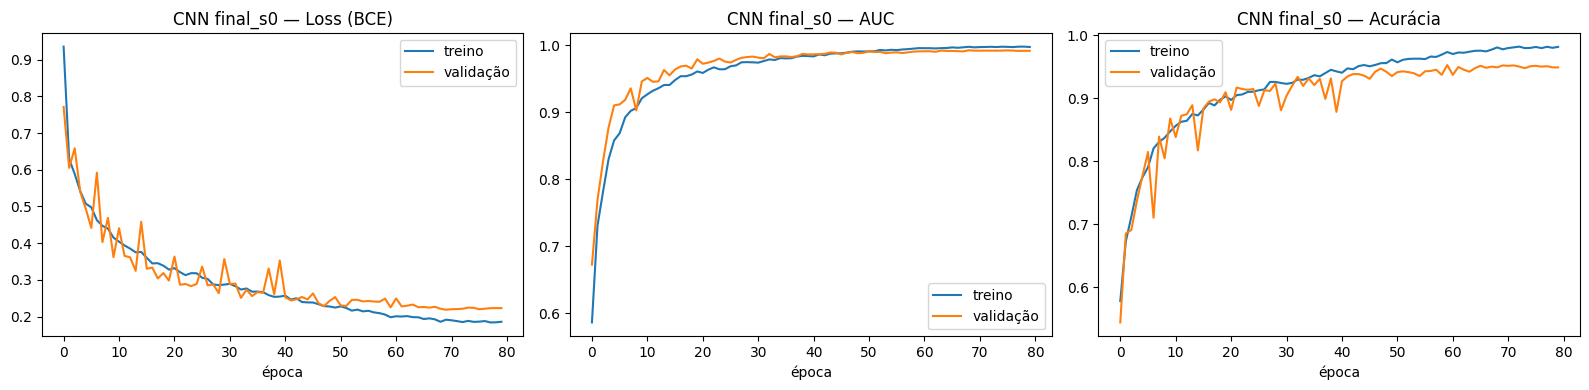
\includegraphics[width=\textwidth]{figuras/treino_s0.png}\\[2pt]
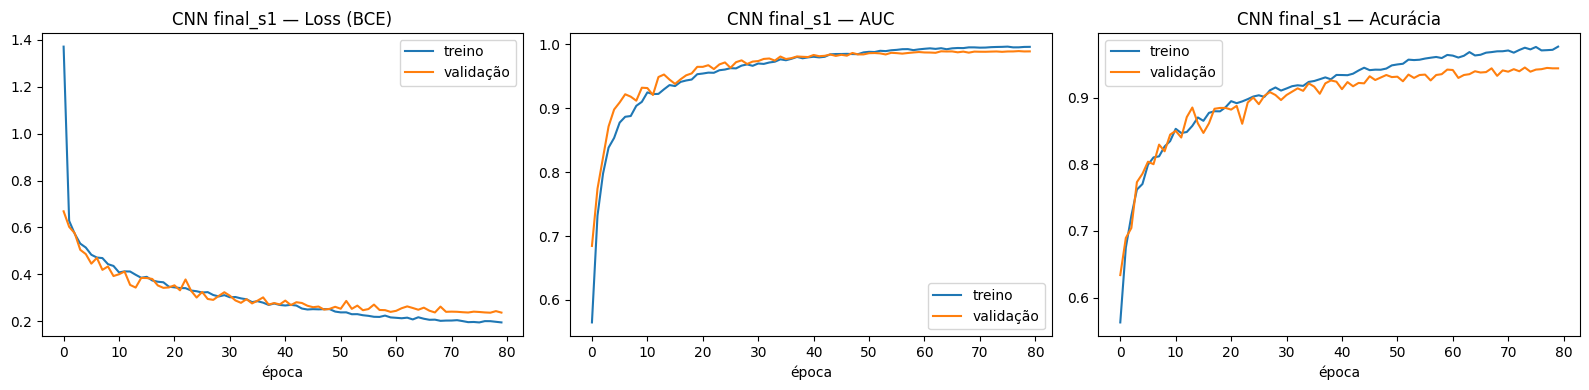
\includegraphics[width=\textwidth]{figuras/treino_s1.png}
\caption{Curvas de perda (entropia cruzada binária), AUC e acurácia por época dos dois modelos do ensemble (sementes 42, acima, e 43, abaixo), no Colab. A validação inclui o conjunto limpo e o degradado.}
\label{fig:treino}
\end{center}
\end{figure*}

\paragraph{Ambiente.} TensorFlow/Keras~\citep{abadi2016tensorflow} 2.21 com GPU NVIDIA no Colab e 2.18 com \texttt{tensorflow-metal} no Mac, librosa~\citep{mcfee2015librosa}, scikit-learn~\citep{pedregosa2011sklearn} e \texttt{ffmpeg}. Durante o projeto foi encontrado um defeito no \texttt{tensorflow-metal} 1.2.0: a sequência Dense $\rightarrow$ bias $\rightarrow$ ReLU devolve valores incorretos na GPU do Mac, com erro de até 0,099 na $P(\text{fake})$. A ReLU foi implementada como \texttt{LeakyReLU} com inclinação zero, matematicamente idêntica e não afetada pelo defeito.

\clearpage % 4.5 começa em página nova, depois das figuras pendentes
\subsection{Métricas e decisão}

A métrica principal é a taxa de erro igual (EER), o ponto da curva ROC em que a taxa de falsos positivos (reais marcados como falsos) é igual à de falsos negativos (falsos aceitos como reais):
\begin{equation}\label{eq:eer}
\text{EER} = \text{FPR}(\tau^{*}) = \text{FNR}(\tau^{*}), \qquad \tau^{*} = \arg\min_{\tau} \left|\text{FPR}(\tau) - \text{FNR}(\tau)\right|.
\end{equation}
Também são relatadas a área sob a curva ROC (AUC), a acurácia, a precisão, o \textit{recall} e o F1.

O limiar de operação é o limiar do EER na validação limpa e degradada, recalculado a cada treino: $\tau = 0{,}573$ no Colab e $\tau = 0{,}475$ no Mac. Um arquivo é classificado como FALSO se $P(\text{fake}) > \tau + 0{,}05$, como REAL se $P(\text{fake}) < \tau - 0{,}05$, e como INCONCLUSIVO entre esses valores.


\section{Experimentos e resultados}
\label{sec:resultados}

\subsection{Protocolo}

Cada mudança no modelo foi avaliada com os mesmos dados antes de ser adotada, segundo uma regra definida antes do experimento. Por exemplo, uma nova arquitetura só substituiria a anterior com ganho de pelo menos 0,5 ponto de EER no teste degradado. O teste degradado aplica ao conjunto de teste as mesmas famílias de degradação do treino (codecs, reenvio pelo WhatsApp, ruído, eco e banda telefônica), com sorteio independente.

\subsection{Resultados do modelo final}

A Tabela~\ref{tab:final} resume o desempenho do ensemble treinado no Colab. O teste de generalização usa apenas sintetizadores que o modelo nunca viu, e mesmo assim o EER fica em 1,25\%. No teste de formato, o mesmo áudio real em WAV, MP3 e Ogg/Opus produziu $P(\text{fake})$ com diferença máxima de 0,001, indicando que o formato do arquivo não é usado como pista.

A Figura~\ref{fig:avaliacao} mostra, para cada conjunto, a matriz de confusão, a curva ROC e a distribuição de $P(\text{fake})$. Nos conjuntos em português, as duas classes ficam concentradas nos extremos. Os erros do teste degradado aparecem como uma cauda de falsos com probabilidade baixa. No In-the-Wild, a distribuição dos falsos se espalha por toda a faixa, e muitos recebem $P(\text{fake})$ próxima de zero.

\begin{figure*}[!ht]
\begin{center}
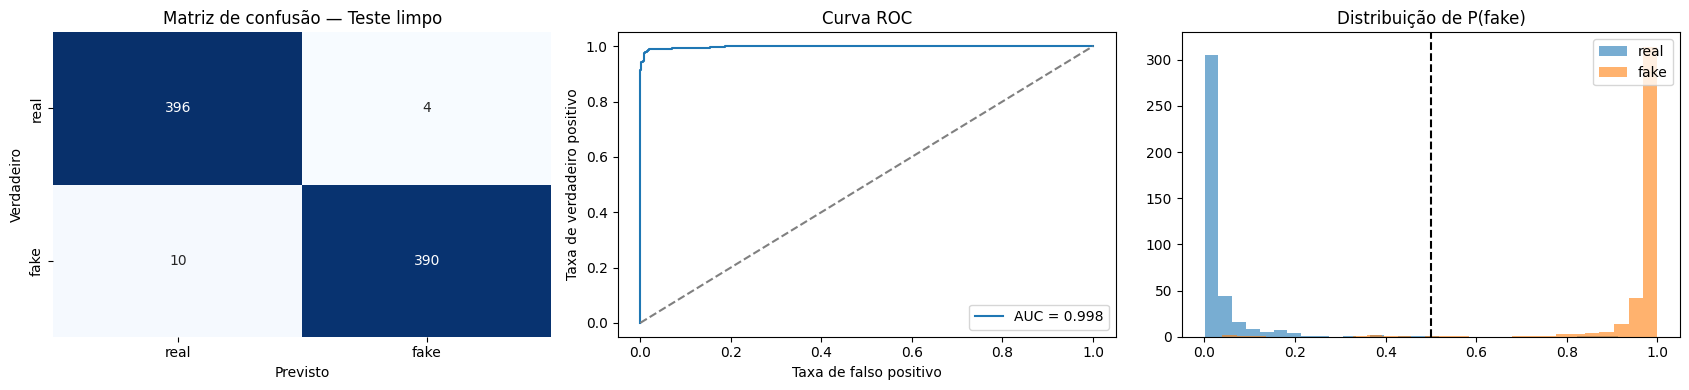
\includegraphics[width=\textwidth]{figuras/avaliacao_limpo.png}\\[2pt]
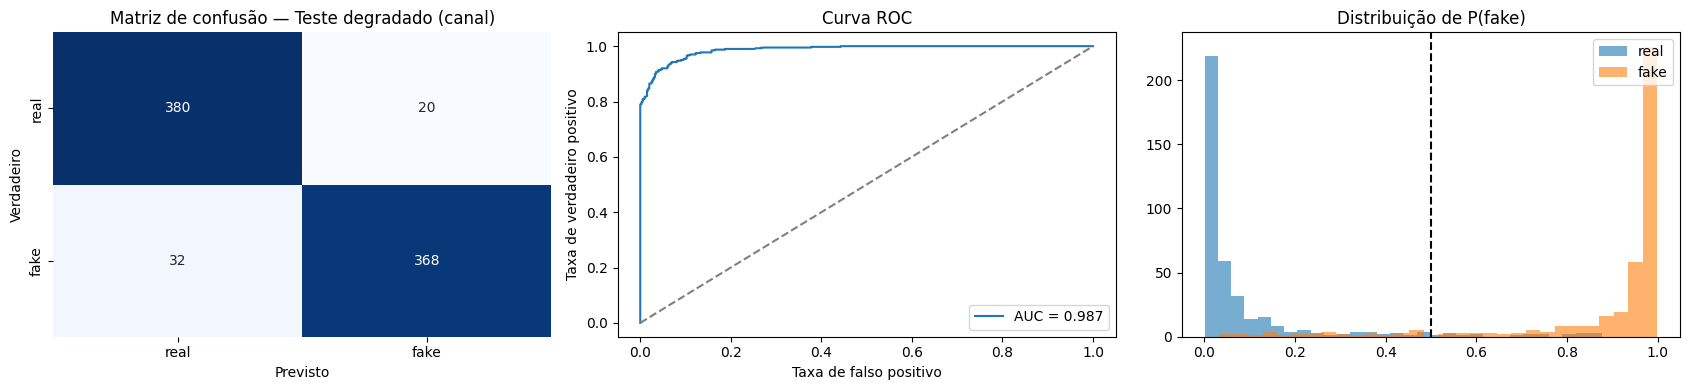
\includegraphics[width=\textwidth]{figuras/avaliacao_degradado.png}\\[2pt]
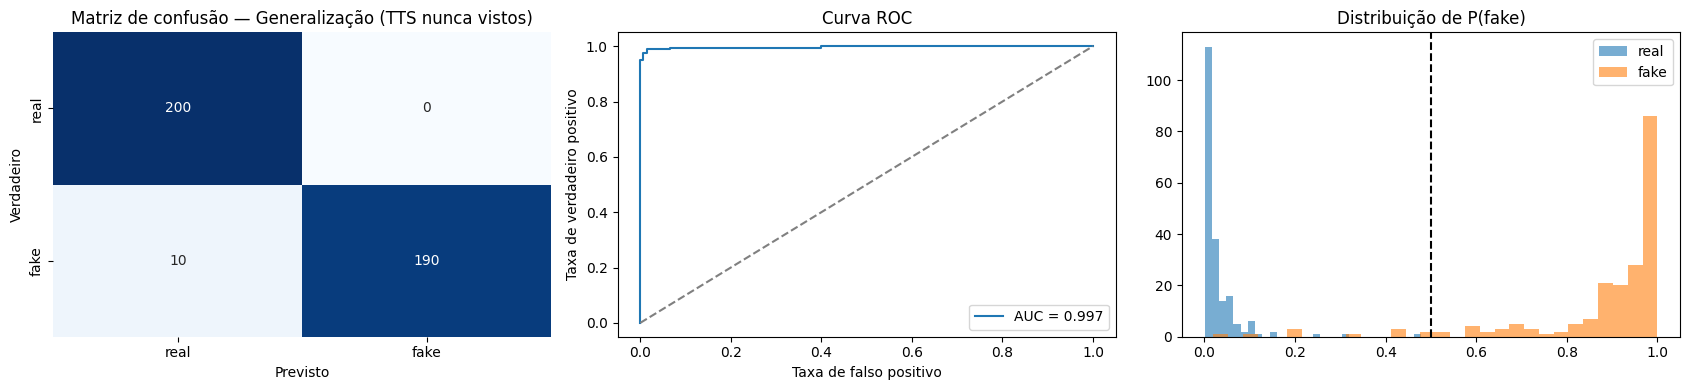
\includegraphics[width=\textwidth]{figuras/avaliacao_generalizacao.png}\\[2pt]
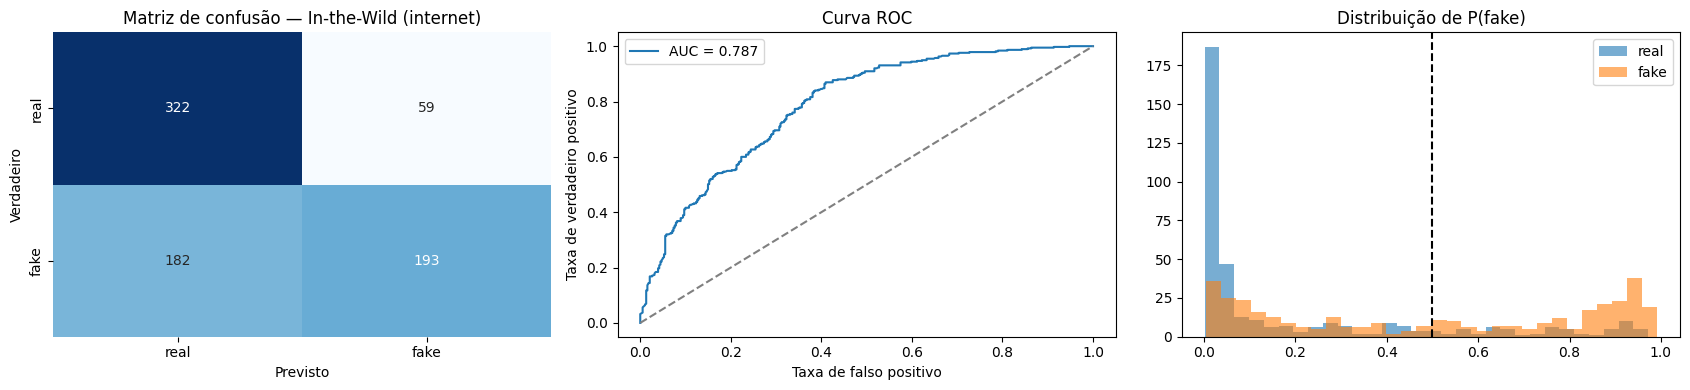
\includegraphics[width=\textwidth]{figuras/avaliacao_in_the_wild.png}
\caption{Avaliação do ensemble no Colab: matriz de confusão, curva ROC e histograma de $P(\text{fake})$ nos testes limpo, degradado, de generalização e In-the-Wild (de cima para baixo). As matrizes e a linha tracejada usam o limiar fixo de 0,5; o limiar de operação (0,573) é usado só na classificação de arquivos.}
\label{fig:avaliacao}
\end{center}
\end{figure*}

\begin{table}[!ht]
\caption{Desempenho do ensemble final (Colab).}
\centering
\small
\begin{tabular}{@{}lccc@{}}
\hline\hline
Conjunto & Acurácia & AUC & EER \\
\hline
Teste limpo & 98,3\% & 0,998 & 1,75\% \\
Teste degradado & 93,5\% & 0,987 & 6,5\% \\
Generalização & 97,5\% & 0,997 & 1,25\% \\
Generalização degradada & 92,0\% & 0,977 & 7,5\% \\
In-the-Wild & 68,1\% & 0,787 & 30,6\% \\
\hline\hline
\end{tabular}
\label{tab:final}
\end{table}

\paragraph{Reprodução em outro ambiente.} A Tabela~\ref{tab:ambientes} compara o mesmo código executado no Colab e no Mac. As bases e as divisões são as mesmas, mas a precisão numérica, o tamanho do lote e a ordem dos sorteios mudam. O Colab teve EER menor no teste limpo e na generalização, e o Mac, no teste degradado. Todas as diferenças ficaram em até 1,8 ponto, e o teste cego teve os mesmos acertos e os mesmos erros nos dois ambientes.

\begin{table}[!ht]
\caption{EER (\%) do ensemble no Colab e no Mac.}
\centering
\small
\begin{tabular}{@{}lcc@{}}
\hline\hline
Conjunto & Colab & Mac \\
\hline
Teste limpo & 1,75 & 3,25 \\
Teste degradado & 6,5 & 4,9 \\
Generalização & 1,25 & 2,5 \\
Generalização degradada & 7,5 & 7,25 \\
In-the-Wild & 30,6 & 28,8 \\
Teste cego (falsos / reais) & 13/16 / 9/9 & 13/16 / 9/9 \\
Tempo de treino & $\approx$36 min & $\approx$4,8 h \\
\hline\hline
\end{tabular}
\label{tab:ambientes}
\end{table}

\paragraph{Teste cego.} Nos 25 áudios do grupo, o modelo do Colab detectou 13 dos 16 falsos e acertou os 9 reais, sem nenhum inconclusivo. Os reais ficaram todos com $P(\text{fake}) \leq 0{,}15$, e os 13 falsos detectados, entre 0,75 e 0,99. Os três falsos não detectados são os mesmos nos dois ambientes: a voz ``Lucas'' do ElevenLabs ($P(\text{fake}) = 0{,}316$ no Colab; 0,431 no Mac) e dois falsos de origem desconhecida reenviados pelo WhatsApp (0,114 e 0,102 no Colab). As metas definidas no início do projeto foram atingidas: EER degradado de no máximo 10\%, generalização de no máximo 20\%, no máximo um real errado no teste cego e pelo menos 80\% dos falsos detectados (13/16 = 81\%).

\paragraph{Classificador.} A última seção do notebook carrega os dois modelos salvos e classifica arquivos enviados pelo usuário. A Figura~\ref{fig:classificador} mostra a saída para uma gravação real de 18~s enviada pelo WhatsApp, que não faz parte do teste cego. As 12 janelas ficaram abaixo de 0,1, e o arquivo foi classificado como REAL, com $P(\text{fake}) = 0{,}026$ e confiança de 97,7\%.

\begin{figure*}[!ht]
\begin{center}
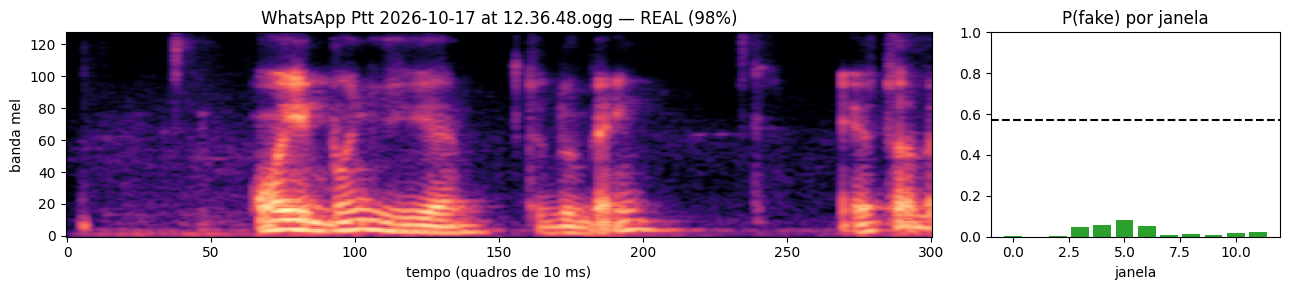
\includegraphics[width=0.9\textwidth]{figuras/classificador_exemplo.png}
\caption{Saída do classificador no Colab para um áudio real do WhatsApp: espectrograma do primeiro trecho e $P(\text{fake})$ de cada janela de 3~s, com o limiar de operação (0,573) tracejado.}
\label{fig:classificador}
\end{center}
\end{figure*}

\subsection{Evolução do modelo}

A Tabela~\ref{tab:evolucao} mostra a evolução ao longo das versões. Os conjuntos de teste mudaram entre algumas versões, por exemplo quando o teste degradado passou a incluir o reenvio pelo WhatsApp, e por isso cada linha só é diretamente comparável à anterior. Os maiores ganhos vieram da troca de LFCC por log-mel, da retirada do BRSpeech-DF e das três versões por áudio com a cadeia do WhatsApp.

\begin{table*}[!ht]
\caption{Evolução do detector (EER, em \%, e acertos no teste cego).}
\centering
\small
\begin{tabular}{@{}p{7.2cm}cccc@{}}
\hline\hline
Versão & Limpo & Degradado & Generalização & Teste cego (falsos / reais) \\
\hline
1ª execução completa (LFCC + BRSpeech-DF) & 28,3 & 30,4 & 14,5 & 7/16 / 4/9 \\
Log-mel, sem BRSpeech-DF, 40 épocas & 4,1 & 14,1 & 10,3 & 12/16 / 9/9 \\
+ 3 versões por áudio e cadeia WhatsApp, 80 épocas & 2,5 & 7,4 & 5,8 & 12/16 / 9/9 \\
+ dados ampliados (8.000 áudios, MLAAD em 5 idiomas) & 3,5 & 6,5 & 4,0 & 13/16 / 9/9 \\
+ arquitetura residual e correção do defeito do Metal & 2,9 & 5,4 & 3,0 & 13/16 / 9/9 \\
+ ensemble de 2 residuais (final) & 3,25 & 4,9 & 2,5 & 13/16 / 9/9 \\
\hline\hline
\end{tabular}
\label{tab:evolucao}
\end{table*}

\subsection{Comparação de arquiteturas}

Quatro arquiteturas e duas variações foram treinadas com os mesmos dados por 20 épocas cada (Tabela~\ref{tab:arquiteturas}). A residual ganhou 3 pontos de EER degradado em relação à CNN original, ao custo de cerca de 2,9 vezes o tempo por época. A LCNN~\citep{lavrentyev2019stc}, o \textit{pooling} por atenção e a entrada mel+LFCC não compensaram.

\begin{table*}[!ht]
\caption{Comparação de arquiteturas (20 épocas, mesmos dados).}
\centering
\small
\begin{tabular}{@{}lllrrcc@{}}
\hline\hline
Arquitetura & Pooling & Entrada & Parâmetros & s/época & EER degradado & EER generalização \\
\hline
Original (4 blocos simples) & média+máx & mel & 155.025 & 38,6 & 12,5\% & 5,0\% \\
\textbf{Residual} & média+máx & mel & 501.953 & 111,6 & \textbf{9,5\%} & 5,0\% \\
LCNN (Max-Feature-Map) & média+máx & mel & 300.321 & 58,9 & 11,25\% & 4,75\% \\
Original & atenção & mel & 155.090 & 39,6 & 11,75\% & 5,75\% \\
Original & média+máx & mel+LFCC & 155.169 & 40,5 & 13,6\% & 4,75\% \\
\hline\hline
\end{tabular}
\label{tab:arquiteturas}
\end{table*}

\subsection{Ensemble}

O ensemble foi adotado por uma regra fixada antes da rodada: ganho de pelo menos 0,5 ponto de EER degradado e teste cego no mínimo igual. A Tabela~\ref{tab:ensemble} mostra que o ensemble reduziu o EER degradado de 5,38\% para 4,88\%, exatamente no limite da regra, e manteve o teste cego. Ele também reduziu a generalização degradada de 9,0\% para 7,25\% e o In-the-Wild de 29,5\% para 28,8\%. Em troca, o EER limpo piorou 0,4 ponto, o tempo de treino dobrou e a classificação passou a executar duas redes. No Colab, o ensemble também foi melhor que cada modelo no teste degradado (6,5\% contra 7,5\% e 6,75\%), mas o ganho sobre o melhor modelo individual foi menor (0,25 ponto).

\begin{table}[!ht]
\caption{EER (\%) de cada modelo e do ensemble, nos dois ambientes.}
\centering
\small
\begin{tabular}{@{}lccc@{}}
\hline\hline
Modelo & Limpo & Degradado & Gener. \\
\hline
\multicolumn{4}{@{}l}{\textit{Mac (rodada de adoção)}} \\
Modelo 0 (semente 42) & 2,88 & 5,38 & 3,0 \\
Modelo 1 (semente 43) & 2,75 & 6,0 & 2,0 \\
\textbf{Ensemble} & 3,25 & \textbf{4,88} & 2,5 \\
\hline
\multicolumn{4}{@{}l}{\textit{Colab}} \\
Modelo 0 (semente 42) & 2,13 & 7,5 & 2,5 \\
Modelo 1 (semente 43) & 1,5 & 6,75 & 1,25 \\
\textbf{Ensemble} & 1,75 & \textbf{6,5} & 1,25 \\
\hline\hline
\end{tabular}
\label{tab:ensemble}
\end{table}

\subsection{Experimentos descartados}
\label{sec:descartados}

\begin{itemize}
\item \textbf{LFCC como entrada:} hipótese inicial, por ser padrão no ASVspoof~\citep{sahidullah2015features}. Com os mesmos dados, o EER degradado foi de 18,5\% contra 12,6\% do log-mel, e o teste cego detectou 10/16 falsos contra 15/16.
\item \textbf{BRSpeech-DF:} seus falsos clonam os mesmos locutores dos reais e confundiam o treino. Retirá-lo levou o EER limpo de 28,2\% para 9,2\% e o degradado de 30,4\% para 18,5\%.
\item \textbf{CNN14 pré-treinada (PANNs)}~\citep{kong2020panns}: reimplementada em Keras com os pesos oficiais, congelada e com uma cabeça densa. Teve EER de 9,9\% (limpo), 20,4\% (degradado) e 14,3\% (generalização), bem atrás da CNN treinada do zero.
\item \textbf{Mixup:} piorou o teste degradado (16,4\% para 17,8\%).
\item \textbf{Adaptação com os áudios do grupo:} com validação cruzada agrupada por voz, chegou a 14/16 falsos e 9/9 reais no teste cego, mas piorou o EER degradado (5,9\% contra 5,4\%). Como o ganho foi de um único arquivo, com apenas 16 vozes, a adaptação não entrou no modelo entregue.
\end{itemize}


\section{Discussão e limitações}
\label{sec:discussao}

Os resultados mostram que a principal causa da falha original era de dados, e não de arquitetura. O modelo nunca tinha visto vozes comerciais e aprendia atalhos como formato, silêncio e locutor. A inclusão de falsos comerciais, o balanceamento de idiomas e a aplicação das mesmas degradações às duas classes explicam a maior parte do ganho. A arquitetura residual e o ensemble trouxeram melhorias menores, mas mensuráveis.

A principal limitação é o desempenho no In-the-Wild (EER de 30,6\% no Colab e 28,8\% no Mac, AUC de 0,79). Esses áudios, em inglês, têm música, muito ruído, gravações antigas e falas espontâneas, um tipo de material que não está no treino, composto por fala lida, entrevistas e TTS. O resultado confirma a observação de \citet{muller2022itw} sobre a distância entre as bases de laboratório e o ``mundo real''.

O teste cego é pequeno: 25 arquivos, quase todos os falsos de um único serviço (ElevenLabs) e todos os reais vindos do WhatsApp. Ele indica o comportamento esperado em uso, mas não permite conclusões estatísticas fortes. Ampliá-lo, com reais gravados fora do WhatsApp e falsos de outros serviços (PlayHT, Murf, Resemble e clonagem da própria voz), é o próximo passo natural. Falsos reenviados várias vezes por aplicativos de mensagem continuam sendo o caso mais difícil.

Por fim, o defeito encontrado no \texttt{tensorflow-metal} distorcia silenciosamente as probabilidades dos modelos treinados antes da correção. Os números das Tabelas~\ref{tab:final}, \ref{tab:arquiteturas} e~\ref{tab:ensemble} já são da versão corrigida. O episódio reforça a importância de comparar a saída da GPU com um cálculo de referência.


\section{Considerações éticas}
\label{sec:etica}

As bases utilizadas são públicas e foram usadas de acordo com suas licenças. O MLAAD, por exemplo, é restrito a uso não comercial, compatível com um trabalho acadêmico. Os áudios do teste cego foram gravados pelos próprios integrantes do grupo, com seu consentimento, ou gerados por eles em serviços de síntese. Esses áudios não são redistribuídos. Nenhuma voz de terceiros foi clonada para este trabalho. O In-the-Wild contém falas de figuras públicas e foi usado apenas para avaliação.

A detecção de deepfakes é uma tecnologia de uso dual: um detector publicado pode ser usado para treinar geradores que o enganem. O detector deste trabalho não deve ser tratado como prova pericial. A faixa INCONCLUSIVA existe justamente para indicar os casos em que a decisão automática não é confiável, e um resultado ``REAL'' não garante que o áudio seja autêntico.


\section{Conclusão}
\label{sec:conclusao}

Este trabalho apresentou um detector de voz deepfake em português brasileiro baseado em um ensemble de duas CNNs residuais treinadas do zero sobre espectrogramas log-mel. No Colab, o modelo atingiu EER de 1,75\% no teste limpo, 6,5\% no teste degradado e 1,25\% em sintetizadores nunca vistos, e detectou 13 de 16 falsos sem errar nenhum dos 9 reais no teste cego com áudios do grupo, resolvendo o problema original de não reconhecer vozes de serviços comerciais.

As decisões que mais contribuíram foram tratar os atalhos nos dados (formato, ruído de fundo, idioma e locutor) e simular as condições reais de uso, como a compressão e o reenvio pelo WhatsApp. Como trabalhos futuros, ficam a ampliação do teste cego, o uso de fala espontânea e ruidosa no treino para reduzir a distância ao In-the-Wild, o ensemble de três modelos e o ajuste fino (\textit{fine-tuning}) de redes pré-treinadas.

O código completo, com treino, avaliação, teste cego e classificador, está disponível como notebook do Google Colab (ver Declarações).


\section*{Declarações}

\begin{contributions}
CERP e FPS conceberam o estudo, implementaram o código, reuniram os áudios do teste cego, executaram os experimentos e escreveram o texto. Ambos os autores leram e aprovaram a versão final.
\end{contributions}

\begin{interests}
Os autores declaram não ter conflitos de interesse.
\end{interests}

\begin{materials}
O código (treino, avaliação, teste cego e classificador) está disponível no Google Colab em \url{https://colab.research.google.com/drive/1HmQv9uw1JC9kW3rhcQowu-Fl1CJYyXn0}. As bases de dados utilizadas são públicas e estão listadas na Tabela~\ref{tab:bases}: MLAAD (\url{https://huggingface.co/datasets/mueller91/MLAAD}), CORAA-MUPE (\url{https://huggingface.co/datasets/nilc-nlp/CORAA-MUPE-ASR}), Common Voice 17 (\url{https://huggingface.co/datasets/fixie-ai/common_voice_17_0}), In-the-Wild (\url{https://huggingface.co/datasets/mueller91/In-The-Wild}) e Deepfake Audio Detection (\url{https://huggingface.co/datasets/garystafford/deepfake-audio-detection}). Os áudios do teste cego, gravados pelo grupo, não são redistribuídos.
\end{materials}


\bibliographystyle{apalike-sol}
\bibliography{refs}

\end{document}
